\chapter{\textit{Cantor Digitalis}, un instrument de synthèse de voyelles chantées}
\label{Sec:CantorDigitalis}
\minitoc
\cleardoublepage

\section{Introduction}
\lipsum[1-2]

\begin{figure}
  \centering
  {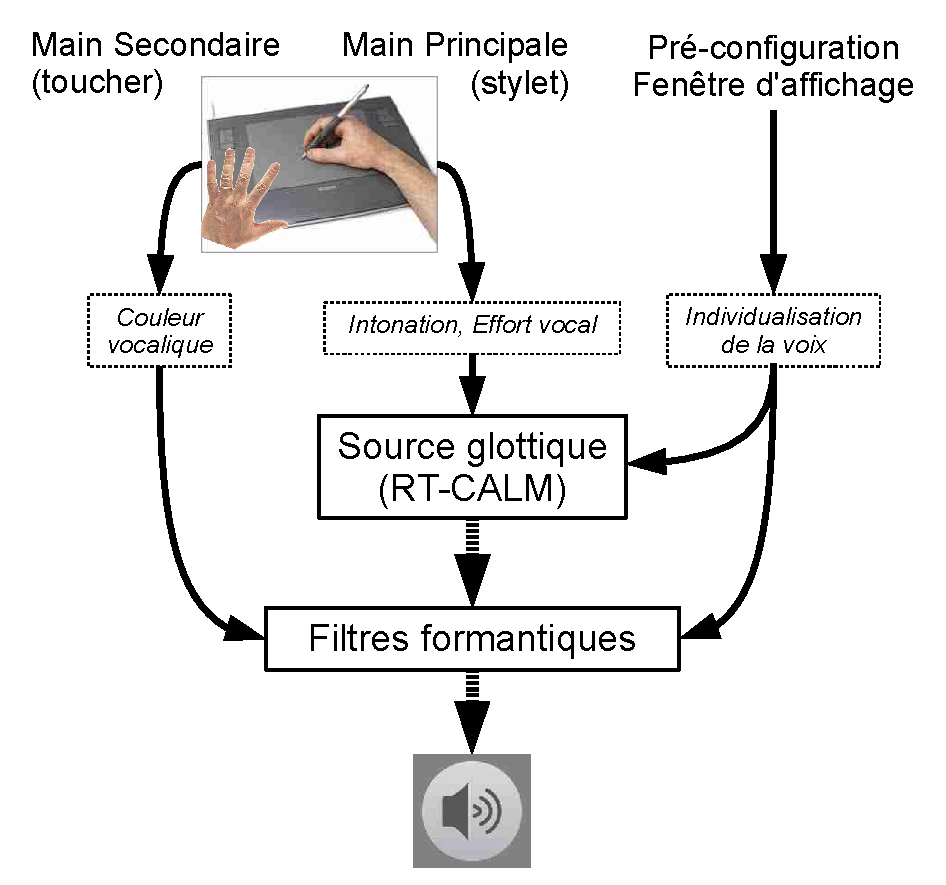
\includegraphics[width=.5\linewidth]{ch2/fig/SchemaFonct_Cantor2.pdf}}
    \caption{{\it Représentation schématique du fonctionnement du synthétiseur Cantor Digitalis}}
  \label{Fig:SchemaFonct_Cantor}
  \hspace{0.3cm}
\end{figure}

\section{Modélisation des résonances du conduit vocal}
\lipsum[1-2]

\subsection{Valeurs des formants des voyelles cibles}
\label{Sec:formantsCibles}
\lipsum[1-1]

\subsection{A propos du formant du chanteur}
\lipsum[1-1]
	
\subsection{Anti-résonance du sinus piriforme}
\lipsum[1-1]

\subsection{Exemple de comparaison entre une voyelle /a/ réelle et de synthèse}
\label{sec:cantor-example-voyelle}
\noindent \textit{Voir fichiers audios~/ vidéos~\ref{fav:natsyn}}\\
\lipsum[1-1]

\section{Dépendances sources-filtres}
\label{Sec:interactionSF}

\lipsum[1-1]


\subsection{Atténuation des résonances en fonction de $F_0$}
\label{sec:cantor-ai-attenuation}
\noindent \textit{Voir fichiers audios~/ vidéos~\ref{fav:ai-attenuation}}\\

\lipsum[1-2]

\subsection{Fréquence du premier formant et effort vocal}
\label{sec:cantor-f1f0}
\noindent \textit{Voir fichiers audios~/ vidéos~\ref{fav:f1-VE-dependance}}\\
\lipsum[1-1]

\subsection{Adaptation des deux premières résonances à $F_0$}
\label{Sec:Fi_F0}
\noindent \textit{Voir fichiers audios~/ vidéos~\ref{fav:fi-f0-dependance}}\\

\lipsum[1-2]



\section{Personnalisation des voix}
\label{Sec:personalisation_voix}



\subsection{Taille du conduit vocal et tessiture}
\label{Sec:tailleConduit}
\noindent \textit{Voir fichiers audios~/ vidéos~\ref{fav:types-voix-1}}\\

\lipsum[1-1]



\subsection{Qualité vocale : de la voix soufflée aux voix monstrueuses}
\label{sec:cantor-voixMonstres}
\noindent \textit{Voir fichiers audios~/ vidéos~\ref{fav:types-voix-2}}\\

\subsection{Volume pulmonaire}


\section{Contrôle gestuel des voyelles chantées synthétiques}
\label{Sec:ctrGestVoy}
\lipsum[1-2]


\subsection{Contrôle du modèle de source glottique}
\lipsum[1-2]


\subsection{Contrôle de l'espace vocalique}
\label{Sec:ControleEspaceVocalique}


\subsubsection{a) Contrôle mono-manuel de la source glottique et du conduit vocal}
\label{Sec:ctrMonoManuel}
\lipsum[1-2]


\subsubsection{b) Contrôle bi-manuel de la source et du conduit vocal}



\subsubsection{c) Contrôle gestuel du chant diphonique}
\label{sec:cantor-chantDiphonique}
\noindent \textit{Voir fichiers audios~/ vidéos~\ref{fav:types-voix-3}}\\

\section{Résumé et conclusions}
\lipsum[1-2]
